\subsection{Farvebilleder}

Synligt lys er eletromagnetisk stråling hvis bølgelængde er i intervallet 400-700nm. Hvor øjet opfatter forskellige bølgelængder som forskellige farver. Som kun er et meget lille del af det elektromagnetiske spectrum.

\begin{figure}[H]
	\centering
	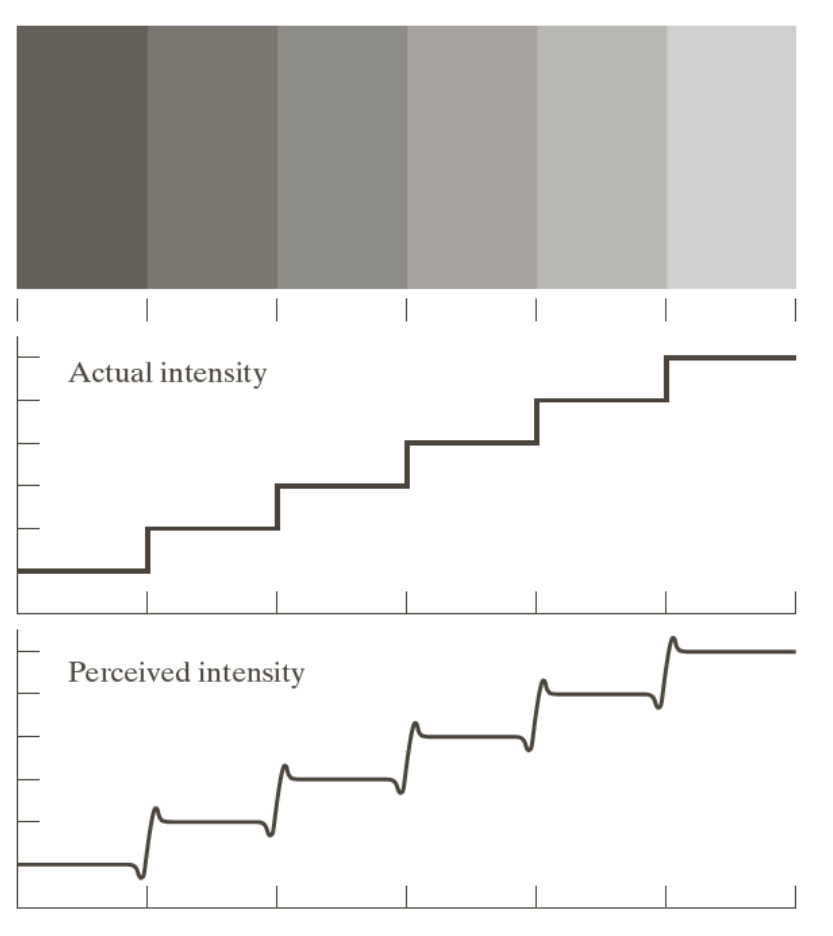
\includegraphics[width=0.7\linewidth]{figs/spm07/mach-band-effect}
	\caption{Mach band effekten.}
	\label{fig:mach-band-effect}
\end{figure}

Figur~\ref{fig:mach-band-effect} viser Mach band effekten, som betyder at selve farven er den samme i et felt, vil menneskets øje alligevel opfatte de modstødende farver som kontraster til hinanden og derfor opfatter vi en ikke-eksisterende gradient.

\subsubsection{Hvidt lys}

En overflade der reflekterer alle synlige bølgelængder ens, synes at være hvidt, mens et objekt der absoberer de fleste bølgelængder udover 500nm-570nm kan syntes grønt.

\subsubsection{Akromatisk lys}

Akromatisk lys er lys uden farve, hvis eneste attribut er intensitet. Intensiteten kan da varieres så det akromatiske lys syntes at være gråtoner.

\subsubsection{Kromatisk lys}

Udover frekvens kan farvet lys beskrives med:

\begin{itemize}
	\item \textbf{Radiance}\\
	Den totale energi i watt.
	
	\item \textbf{Luminance}\\
	Mængden af energi som en observer ser.
	
	\item \textbf{Brightness}\\
	Lidt ligesom intensitet. Er en subjektiv beskrivelse som ikke kan måles.
\end{itemize}

\textbf{\textit{Cones}} i øjet, er de sensorer som giver os evnen til at opfatte farver.\\
Disse deles op i tre kategorier, alt efter hvad de er følsomme overfor: rød, grøn eller blå. RGB er primærfarverne. 

\subsubsection{Farve karakteristika}

Tre attributter, som vi bruger til at karakterisere farve med: 

\begin{itemize}
	\item \textbf{Brightness}\\
	Lidt ligesom intensitet. Er en subjektiv beskrivelse som ikke kan måles.
	
	\item \textbf{Hue}\\
	Beskriver den dominerende bølgelængde. Renheden af den enkelte farve.
	
	\item \textbf{Saturation}\\
	Beskriver hvor meget hvidt lys der er i farven.
\end{itemize}
